% include all necessary latex libraries
\documentclass[aspectratio=169,presentation]{beamer}
\usetheme{Boadilla}
\useinnertheme{default}

% -- locale-setup --------------------------------------------------------------

\usepackage[utf8]{inputenc}
\usepackage[T1]{fontenc}
\usepackage[ngerman]{babel}
\usepackage{lmodern}
\usepackage[locale=DE, mode=math, list-final-separator={ oder },
            range-phrase={ bis }, scientific-notation=false, 
            group-digits=integer] {siunitx}

% -- package-includes ----------------------------------------------------------

\usepackage{tikz}
\usepackage{xcolor}
\usetikzlibrary{positioning,automata,matrix,arrows.meta,fit}
\usepackage{graphicx} % including images
\usepackage[font=small,labelfont=bf]{caption} % captions of tables and figures

% -- listing setup -------------------------------------------------------------

\usepackage{listings}
\definecolor{pblue}{rgb}{0.13,0.13,1}
\definecolor{pgreen}{rgb}{0,0.5,0}
\definecolor{pred}{rgb}{0.9,0,0}
\definecolor{pgrey}{rgb}{0.46,0.45,0.48}
\definecolor{javared}{rgb}{0.6,0,0} % for strings
\definecolor{javagreen}{rgb}{0.25,0.5,0.35} % comments
\definecolor{javapurple}{rgb}{0.5,0,0.35} % keywords
\definecolor{javadocblue}{rgb}{0.25,0.35,0.75} % javadoc

\lstset{language=vhdl,
	basicstyle=\ttfamily,
	keywordstyle=\color{javapurple}\bfseries,
	stringstyle=\color{javared},
	commentstyle=\color{javagreen},
	morecomment=[s][\color{javadocblue}]{/**}{*/},
	tabsize=2,
	showspaces=false,
	showstringspaces=false
}

% -- custom commands -----------------------------------------------------------

% just prints given text in large text and on empty frame.
\newcommand{\sectionframe} [1] {
	\begin{frame}
		\vfill
		\Huge
		\centering
		\usebeamercolor[fg]{title}
		#1
		\vfill
		\par
	\end{frame}
}

% wrapper-command to make pretty title takes
% 1=short-title 2=long-title 3=terminnumber 4=date
\newcommand{\maketitlepage} [5] {
  \title[#1]{#2}
  \subtitle{Termin #3}
  \date{#4}
  \author[Jakob Otto]{Jakob Otto}
  \institute{HAW Hamburg}
  \subject{#1}
  \pgfdeclareimage[height=0.5cm, width=1.3cm]{university-logo}{#5}
  \logo{\href{https://www.haw-hamburg.de}{\pgfuseimage{university-logo}}}
  \begin{frame} {}
    \titlepage
  \end{frame}
}

% draws a link symbol
\newcommand{\externalLink} {
  \tikz[x=1.2ex, y=1.2ex, baseline=-0.05ex]{
    \begin{scope}[x=1ex, y=1ex]
      \clip (-0.1,-0.1) 
        --++ (-0, 1.2) 
        --++ (0.6, 0) 
        --++ (0, -0.6) 
        --++ (0.6, 0) 
        --++ (0, -1);
      \path[draw, 
        line width = 0.5, 
        rounded corners=0.5] 
      (0,0) rectangle (1,1);
    \end{scope}
      \path[draw, line width = 0.5] (0.5, 0.5) 
        -- (1, 1);
    \path[draw, line width = 0.5] (0.6, 1) 
      -- (1, 1) -- (1, 0.6);
  }
}

% Adds a circled number -> Looks better than the default
\newcommand{\circled} [1] {
  \tikz[baseline=(char.base)]{
    \node[shape=circle,draw,inner sep=2pt, text centered, text width = .2cm] (char) {#1};
  }
}

% -- extra includes go here ----------------------------------------------------
\usepackage{tikz}
\usepackage[customcolors]{hf-tikz}
\usetikzlibrary{shapes,arrows, positioning, fit, backgrounds}

\newcommand{\connectlr} [3] {
  \path (#1.east) -- (#1.north east) coordinate[pos=0.5] (tmp11);
  \path (#2.west) -- (#2.north west) coordinate[pos=0.5] (tmp21);
  \draw[-latex] (tmp21) -- (tmp11);
  \path (#1.east) -- (#1.south east) coordinate[pos=0.5] (tmp12);
  \path (#2.west) -- (#2.south west) coordinate[pos=0.5] (tmp22);
  \draw[-latex] (tmp12) -- (tmp22);
  \path (#1) -- (#2) node [midway] {\circled{#3}};
}

\newcommand{\connecttb} [3] {  
  \path (#1.south) -- (#1.south west) coordinate[pos=0.5] (tmp11);
  \path (#2.north) -- (#2.north west) coordinate[pos=0.5] (tmp21);
  \draw[-latex] (tmp21) -- (tmp11);
  \path (#1.south) -- (#1.south east) coordinate[pos=0.5] (tmp12);
  \path (#2.north) -- (#2.north east) coordinate[pos=0.5] (tmp22);
  \draw[-latex] (tmp12) -- (tmp22);
  \path (#1) -- (#2) node [midway] {\circled{#3}};
}

% put color to \boxed math command
\newcommand*{\boxcolor}{orange}
\makeatletter
\renewcommand{\boxed}[2]{\textcolor{#1}{%
\tikz[baseline={([yshift=-1ex]current bounding box.center)}] \node [rectangle, minimum width=1ex,rounded corners,draw] {\normalcolor\m@th$\displaystyle#2$};}}
 \makeatother

%-------------------------------------------------------------------------------
%	Variablen
%-------------------------------------------------------------------------------

\newcommand{\terminnumber}{7}
\newcommand{\hawlogo}{../presentation-template/figs/logo-haw-2017}
\newcommand{\kratzen}{../presentation-template/figs/kratzen}
\newcommand{\aufgabenzettellink}{https://users.informatik.haw-hamburg.de/~schafers/LOCAL/S19W_CE/Aufgabenzettel_Nr4_v12.pdf}

%-------------------------------------------------------------------------------
%	Dokument
%-------------------------------------------------------------------------------

\begin{document}
  \maketitlepage {CE Tutorium} {Tutorium zu\\Computer-Engineering\\im WS19}
  {\terminnumber} {\today} {\hawlogo}

  %---------------------------------------------------------------------------------------------------------------------
  %	Ablauf
  %---------------------------------------------------------------------------------------------------------------------
  \section{Was steht an?}
  \begin{frame}{Ablauf}
    \begin{columns}
      \column{0.6\textwidth}
      \begin{itemize}
        \item Neue Aufgabe
        \item SPI
        \item Flash-Speicher
      \end{itemize}
      \column{0.4\textwidth}
      
\includegraphics[width=0.6\textwidth]{\kratzen}
    \end{columns}
  \end{frame}

  %---------------------------------------------------------------------------------------------------------------------
  %	Ideen für Aufgabe 1
  %---------------------------------------------------------------------------------------------------------------------


  \sectionframe{\link{\aufgabenzettellink}{Aufgabenzettel}}

  \section{SPI}
  \sectionframe{\link{https://users.informatik.haw-hamburg.de/~schafers/LOCAL/S19W_CE/DOCU/uC Reference Manual RM0090 DM00031020 DocID_018909_Rev14 2017-04.pdf}{SPI Dokumentation}}

  \begin{frame} {SPI (I)}
    \begin{block} {Was ist das?}
      \begin{itemize}
        \item Kommunikationsprotokoll für Hardwarebausteine
        \item Master-Slave orientiertes Modell
        \item Full-Duplex - gleichzeitig in beide Richtungen
      \end{itemize}
    \end{block}
  \end{frame}

  \begin{frame} {SPI (II)}
    \begin{block} {Wichtige SPI-pins}
      \begin{itemize}
        \item CS ~~~~- Chip-Select
        \item SCLK - Serial Clock
        \item MOSI - Master Out Slave In
        \item MISO - Master In Slave Out
      \end{itemize}
    \end{block}
  \end{frame}

  \begin{frame} {SPI (III)}
    \begin{center}
      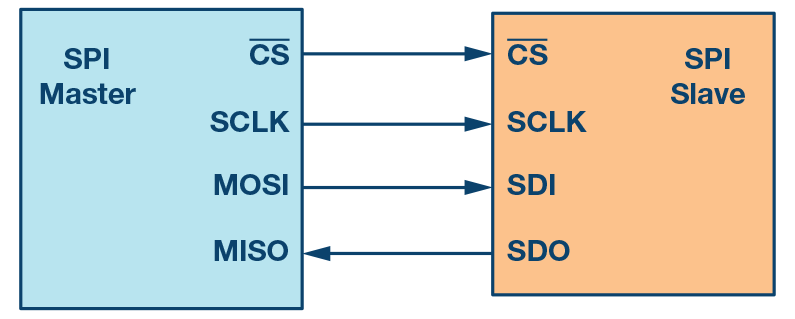
\includegraphics[width=.8\textwidth]{figs/SPI-single.png}
    \end{center}
  \end{frame}

  \begin{frame} {SPI (IV)}
    \begin{center}
      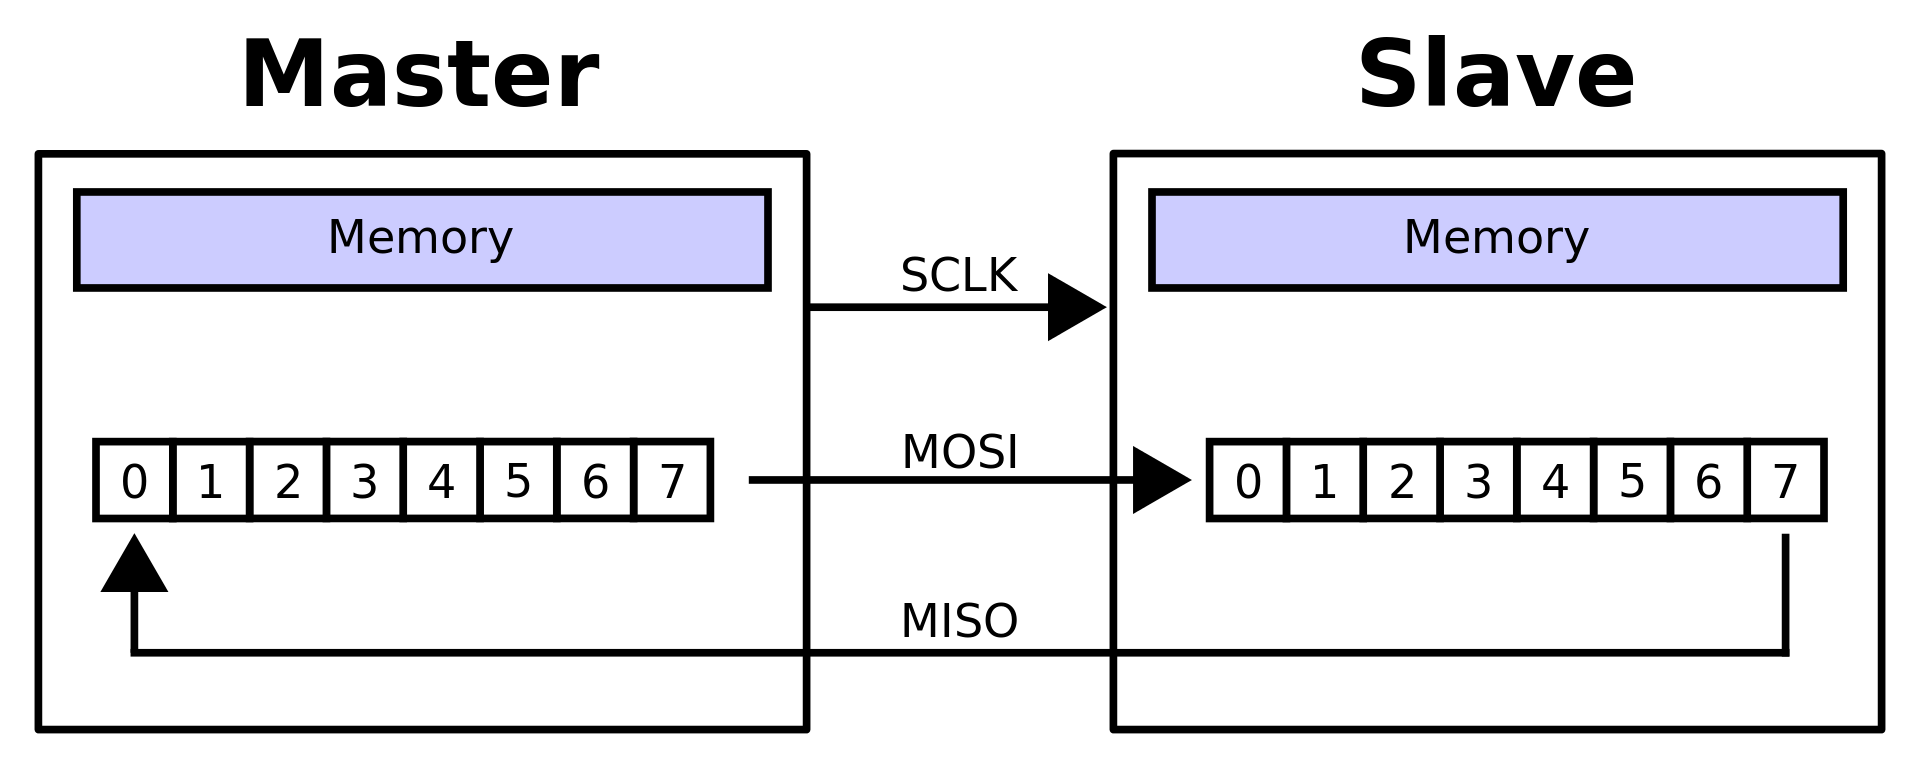
\includegraphics[width=\textwidth]{figs/SPI-transfer}
    \end{center}
  \end{frame}

  \begin{frame} {SPI (V)}
   \begin{block} {Funktionsweise}
      \begin{itemize}
        \item Master gibt takt vor
        \item Slave nutzt Takt um Dinge zu tun
        \item Pro tick wird ein bit übermittelt
      \end{itemize}
    \end{block}
    \begin{alertblock} {}
      Dies passiert im tausch!
    \end{alertblock}
  \end{frame}

  \begin{frame} {SPI (VI)}
    \begin{block} {}
    \begin{itemize}
      \item SPI lässt auch mehrere Slaves zu
      \item CS pin wählt einen Slave zur Zeit
      \begin{itemize}
        \item[$\rightarrow$] Wichtig für die Aufgabe.
      \end{itemize}
    \end{itemize}
  \end{block}
  \end{frame}

  \begin{frame} {SPI}
    \begin{center}
      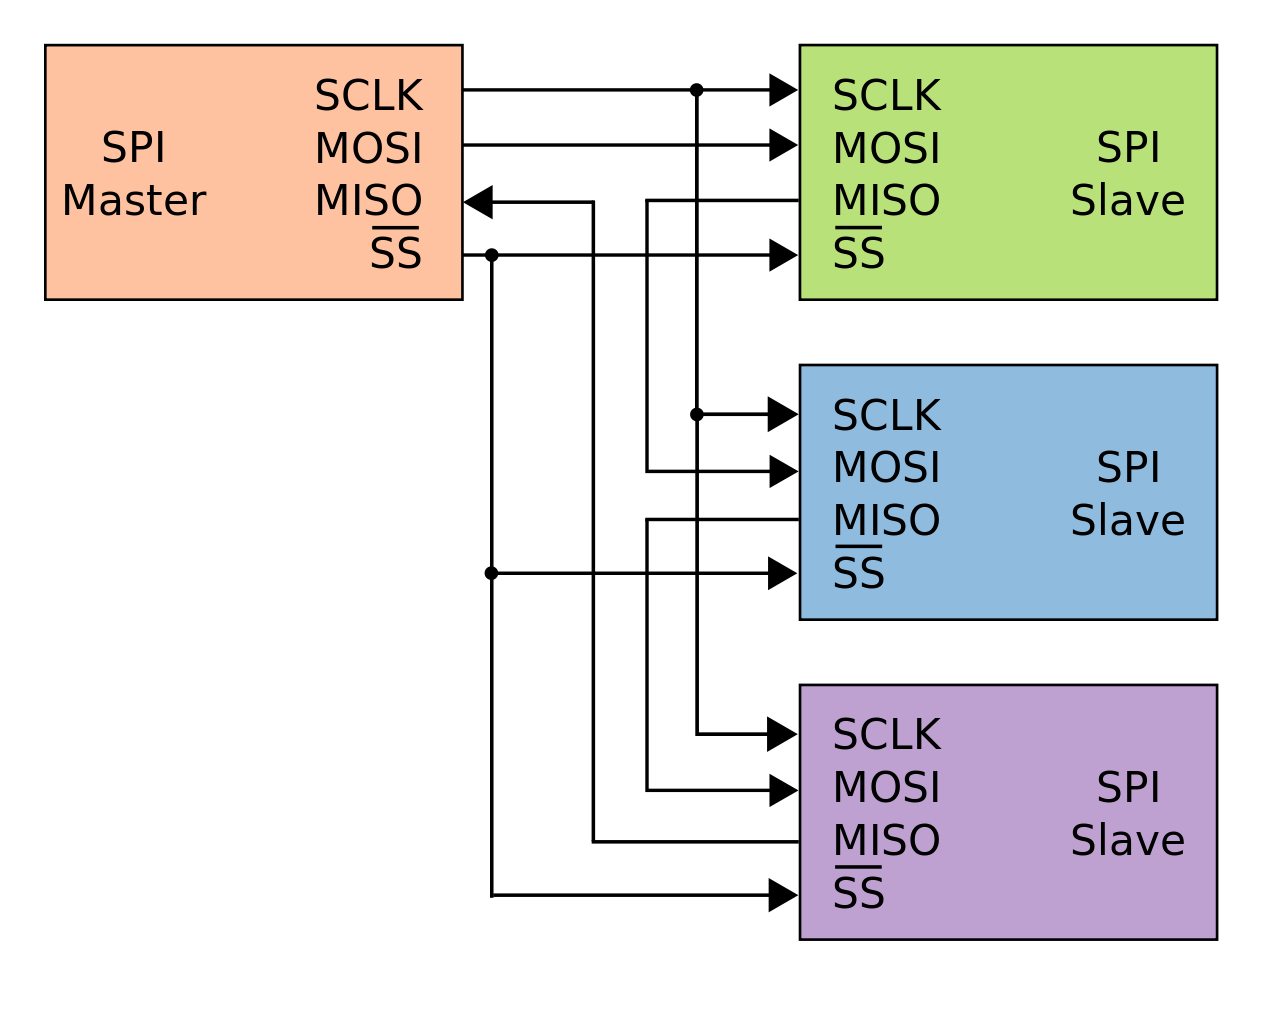
\includegraphics[height=.8\textheight]{figs/SPI-daisychain}
    \end{center}
  \end{frame}

  \begin{frame} {SPI}
    \begin{center}
      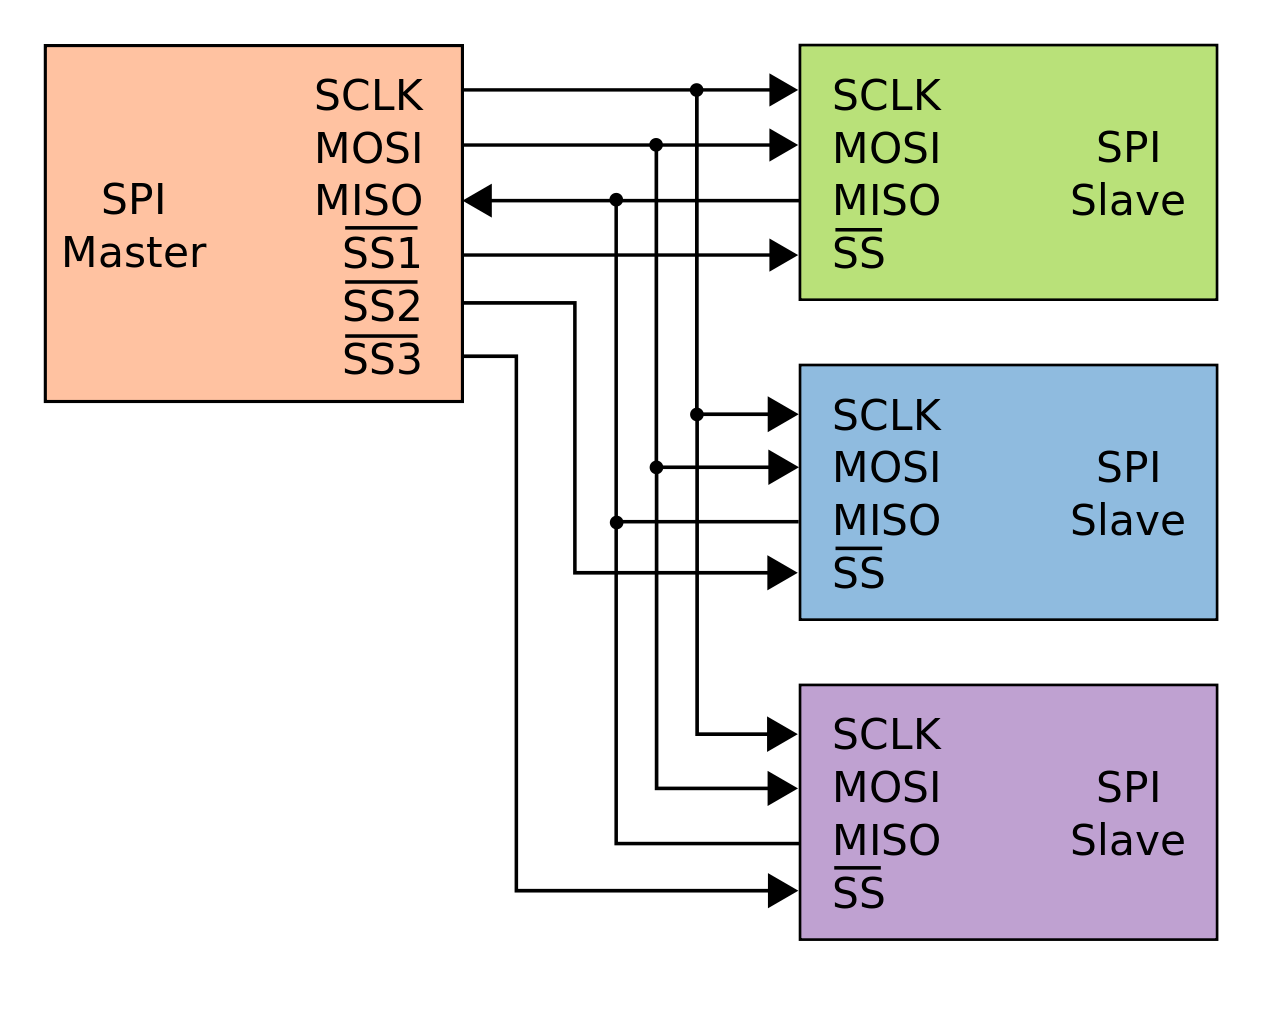
\includegraphics[height=.8\textheight]{figs/SPI-parallel}    
    \end{center}
  \end{frame}

  \begin{frame} [fragile] {STM32-SPI}
    \begin{itemize}
      \item SPI ist in Hardware vorhanden
      \item lesen/schreiben:
      \begin{enumerate}
        \item Byte in Dataregister schreiben
        \item Auf Übertragungsende warten
        \item Empfangene Daten zurückgeben
      \end{enumerate}
      \begin{lstlisting}
uint8_t spi_write_byte(uint8_t data) {
  SPI3->DR = data;
  while(!(SPI3->SR & SPI_SR_RXNE)); 
  return SPI3->DR;
}
        \end{lstlisting}
    \end{itemize}
  \end{frame}

  \sectionframe{\link{https://users.informatik.haw-hamburg.de/~schafers/LOCAL/S19W_CE/CODE/DemoForLabA4_SPI/main.c}{Beispielcode}}  

  \section{Flash-Memory}
  \sectionframe{\link{{https://users.informatik.haw-hamburg.de/~schafers/LOCAL/S19W_CE/DOCU/AT25DF641 Atmel 64MB SPI Serial Flash Memory Datasheet.pdf}}{Flash-Memory-Datasheet}}

  \sectionframe{In der \link{https://owncloud.informatik.haw-hamburg.de}{\color{red}{owncloud}} gibts was einfacheres}

\end{document}